\section{Background research} 

\subsection{Argumentation Theory: General introduction}
This section is mostly based on Dung's theory of argumentation \cite{Dung1995321}. 

\begin{definition}
	An argumentation framework is a tuple $AF = \langle S, R \rangle$ where $S$ is a set of arguments and $ R \subseteq S \times S$. $R$ is called the attack relation.
\end{definition}

An (abstract) argumentation framework can be represented as a directed graph, nodes being arguments, arrows between node $A$ and $B$ representing an attack from argument $A$ to $B$. \autoref{fig:small_af} represents an argumentation framework with the definition $AF = \langle \{A, B, C\}, \{(A,B), (A, C), (B, A), (B, B), (B, C) \}\rangle$.

\begin{notation}
In this paper we use capital letters $A, B, $ to denote arguments. $AB$ denotes an attack from $A$ to $B$ ($(A,B) \in R$).	
\end{notation}

For the following definitions let $AF=\langle S, R \rangle, S' \subseteq S$.

\begin{definition}
 A subset $S'$ is \textbf{conflict free} iff $ \forall A, B \in S': (A, B) \notin R$ \textit{(the subset has not attacks between its arguments)}.
\end{definition}

\begin{definition}
A set $ S' \subseteq S$ \textbf{defends} an argument $A \in S$ iff $\forall B \in S; (B, A) \in R \Rightarrow \exists C \in S': (C, B) \in R$ \textit{(a set $S'$ defends an argument $B \in S$ iff for every argument $B \in S$ that attacks $A$ there is an element $C \in S'$ such that $C$ attacks $B$).}
\end{definition}


\begin{definition}
$A$ is \textbf{acceptable} with respect to a subset $S'$ iff  $\forall B \in S: (B, A) \in R \Rightarrow \exists C \in S': (C, B) \in R$ \textit{(an argument $A$ is acceptable under a subset $S'$ if for each attacker of $A$ there is an argument in $S'$ that attacks these attackers of $A$)}.
\end{definition}

\begin{definition}
	A set $S' \subseteq S$ is \textbf{admissable} if $A$ is conflict-free and defends all of its arguments.
\end{definition}



\begin{definition}
complete extension	
\end{definition}

\begin{definition}
grounded extension	
\end{definition}

\begin{definition}
prefered extension	
\end{definition}

\begin{definition}
stable extension	
\end{definition}

\begin{definition}
	Acaptability of arguments under an extension
\end{definition}



\begin{figure}[h]
\centering
\begin{tikzpicture}[->,>=stealth',shorten >=1pt,auto,node distance=3cm,
                    thick,main node/.style={circle,draw,font=\sffamily\Large\bfseries}]

  \node[main node] (A) {A};
  \node[main node] (B) [below left of=A] {B};
  \node[main node] (C) [below right of=A] {C};
  
  \path[every node/.style={font=\sffamily\small}]
    (A) edge [bend right] node [left] {} (B)
        edge node [left] {} (C)
    (B) edge [bend right] node [left] {} (A)
        edge node [left] {} (C)
        edge [loop left] node {} (B)
     ;
\end{tikzpicture}
\caption{Small example argumentation framework}
\label{fig:small_af}
\end{figure}








%%%%%%%%%%%%%%%%%%
\bigskip
\hrule	
\bigskip



Fundamental mechanism, humans use in argumentation, and exploring ways to implement this mechanism on computers. 
\begin{itemize}
	\item developing a theory for argumentation (central notion is the acceptability of arguments) \cite{Dung1995321}, \cite{Modgil2009}
	\item correctness of this theory ( most approaches to nonmonotonic reasoning in AI and logic programming are special forms of this theory of argumentation)
	\item appropriateness of this theory (illustrates how our theory can be used to investigate the logical structure of many practical problems)
\end{itemize}
Mostly based on Dung\cite{Dung1995321}. Biggest difference: we argue with inconsistent SKB so defeasible argumentation. 

Liao \cite[Chapter 2]{liao} provides the same semantic of argumenatation. Just introducing extension based and labelling based approach. Pointing out differences.

\subsection{Argumentation Theory - Working with Preferences in AF}
Based on Isabel's second paper\cite{sassoon2016}, based on Extended Argumentation Framework\cite{Modgil2009}, using preferences as arguments for attacks on the attack-relation in the original argumentation.
Distinguishing to Amgouds's\cite{amgoud}  Preference based Argumentation Framework.

\subsection{Source paper}
Short summary of Isabels paper \cite{sassoon2014}. Focus on argumentation theory behind it and model selection process. Preferences expressed as attacks on the attacks between the arguments for models.

\subsection{Related work}
\begin{itemize}
	\item Argumentation for Aggregating Clinical Evidence \cite{hunter}: multiple outcome indicators, checks only old date, not supposed data for recommendation, focuses on generation of arguments out of evidence
	\item An argument-based approach to reasoning with clinical knowledge\cite{Gorogiannis20091}: Focus on simple language representing the results of clinical trials, doesn't deal with preferences of different priorities.
	\item In Argumentation for Decision Support\cite{Atkinson2006} an approach using values in the AF is presented, where $A2$ defeats $A1$ iff $A2$ attacks $A1$ and $val(A2) \ngtr_a val(A1)$ which is not applicable as no strict partial order given.
\end{itemize}


\section{Design process - Use Cases}
Taken from Ivar Jacobson, see \autoref{fig:usecase20:flow}.\insertref{UseCase2.0}
\begin{itemize}
	\item popular MoSCoW (Must, Should, Could, Would) prioritization scheme
	\item Use Case on one card (Priority, Release, Size, Complexity)
	\item Use Case Slices generated from use case (Flows, Tests, Estimation)
	\item Find Actors and Use Cases (slice them subsequently)
	\item Prepare Use Case Slices by describing related stories (use-case narrative) and defining test cases
	\item Analyse Use Case Slices (check how the system elements will interact to perform the use case)
	\item Implement Use Case Slice
	\item Test Use Case Slice
	\item Inspect and Adapt
	\item Test System
\end{itemize}



\begin{figure}[!ht]
\centering
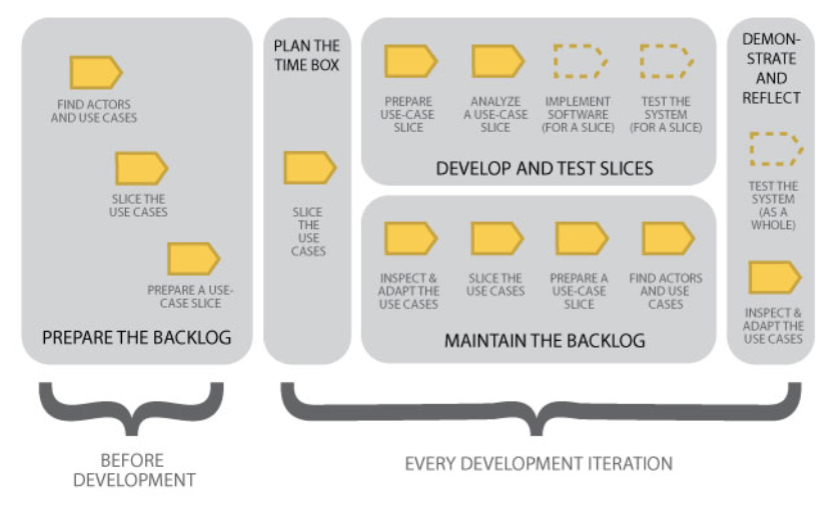
\includegraphics[width=0.8\textwidth]{figures/uc20_flow}
\caption{Use-case 2.0 activities for iterative development approaches}
\label{fig:usecase20:flow}
\end{figure}


\section{Involved Data}
\subsection{Actual data}
The data makes use of a small data set used to illustrate the use of survival analysis methodologies when teaching the subject. The data set is called ovarian and contains the survival in a randomised trial comparing two treatments for ovarian cancer. This has 26 cases and the following columns:
\begin{itemize}

\item futime: survival\footnote{Survival in days while not observing the event} or censoring time\footnote{Patient left the observation after this amount of time and the event didnt take place}
\item fustat: censoring status (1: survival, 0: censored\todo{Is this like this?})
\item age: of the patient in years
\item resid.ds: residual disease present (1=no,2=yes) 
\item rx: treatment group (integers)
\item ecog.ps: ECOG performance status (see \autoref{tab:ecog})
\end{itemize}

\subsection{Statistical Knowledge Base}
\begin{itemize}
	\item Models are suitable for research questions
	\item models have critical assumptions
	\item Models have non-critical assumptions (might be violated and can still be alright to use
	\item \texttt{m2 must fulfil the following critical assumptions ["a1", "a2"], ... }\insertref{Isabels follow up paper of example and data and models}
	\item \texttt{ Survival can be achieved by using the following model \{"m1"=>"a1", "m2"=>["a1", "a2"], "m3" =>["a1", "a3"]\}}
	\item Assumptions met given ($a_i$). Then we use AS1 ($m_i$ is a possible model if 
			\footnote{
				- Model $m_i$ achieves objective $o_c$\\
				- The data set meets the set of assumptions $A_t' = A_t (m_i)$\\
				- The research project meets the set of assumptions $A'_q = A_q (m_i)$\\
				- $A_c(m_i) \subseteq A_t' \cup A_q'$\\
				- $A_t$: Tests are assumptions that are assessed by applying a test on the available data set \\
				- $A_q$: queries are assumptions that are assessed by asking the clinician for an opinion.
			})
	\item R-Code (execution in Ruby possible \cite{rinRuby}  \insertref{https://github.com/clbustos/rinruby} \footnote{\texttt{rinruby} is a gem, that enables evaluation of R code in ruby}) and required outcomes for it decide, whether this model $m_i$ is possible or not. 
\end{itemize}
